%%%%%%%%%%%%%%%%%%%%%%%%%%%%%%%%%%%%%%%%%%%
%
% Document class
%
% Change this if you want a different size/orientation poster etc.
%
%%%%%%%%%%%%%%%%%%%%%%%%%%%%%%%%%%%%%%%%%%%

%\documentclass[landscape,a0b,final,a4resizeable]{a0poster}
%\documentclass[portrait,a0b,final,a4resizeable]{a0poster}
%\documentclass[portrait,a0b,final]{a0poster}
\documentclass[portrait,a0b,final]{a0poster}

\usepackage{etex}

%%%%%%%%%%%%%%%%%%%%%%%%%%%%%%%%%%%%%%%%%%%
%
% Basic packages
%
%%%%%%%%%%%%%%%%%%%%%%%%%%%%%%%%%%%%%%%%%%%

\usepackage{multicol}
\usepackage{color}
\usepackage{shadow}
\usepackage{morefloats}
\usepackage[pdftex]{graphicx}
\usepackage{rotating}
\usepackage{amsmath, amsthm, amssymb, amsfonts}
\usepackage{amsfonts,dsfont}
\usepackage{array}
\usepackage{nth}
\usepackage{booktabs}
\usepackage{bbm}
\usepackage{verbatim}
\usepackage{graphicx}
\usepackage{tikz}
\usetikzlibrary{positioning}


% To use the framed environment 
\usepackage{framed} 

% Bibliography without title.
\usepackage[square, numbers, comma]{natbib}
\renewcommand{\bibsection}{}

% Caption for use outside floats.
\newcommand{\myCaption}[1]{\parbox{\linewidth}{\large \vspace{10pt} #1 \vspace{10pt}}}

% Subfigures, etc.
\usepackage{subfigure}

%\usepackage{pagegrid}
\usepackage{eucal}

% My maths macros.
%\usepackage{mathsMacros}

% Orange emphasis.
\newcommand{\oEmph}[1]{\textcolor{orange}{#1}}

% My commands.
\newcommand{\Exponential}{\mathrm{Exp}}
\newcommand{\diff}{\mathrm{d}}
\newcommand{\grad}{\nabla}
\newcommand{\Ind}{\mathbb{I}}
\newcommand{\Uniform}{\mathrm{Uniform}}
\newcommand{\lambdaref}{\lambda_{\text{ref}}}

%%%%%%%%%%%%%%%%%%%%%%%%%%%%%%%%%%%%%%%%%%%
%
% TIKZ packages and common definitions
%
% Add extra things as per your tikz needs
%
%%%%%%%%%%%%%%%%%%%%%%%%%%%%%%%%%%%%%%%%%%%

\usepackage{picins}
\usepackage{tikz}
\usetikzlibrary{shapes.geometric,arrows,chains,matrix,positioning,scopes,calc}
\tikzstyle{mybox} = [draw=white, rectangle]

\graphicspath{{PosterFigures/}{PaperFigures/}{Branding/}}

%%%%%%%%%%%%%%%%%%%%%%%%%%%%%%%%%%%%%%%%%%%
%
% Some standard colours
%
%%%%%%%%%%%%%%%%%%%%%%%%%%%%%%%%%%%%%%%%%%%

\definecolor{oxdarkblue}{cmyk}{1, 0.8, 0, 0.6}
\definecolor{lightblue}{rgb}{0, 0, 0.80}
\definecolor{white}{rgb}{1, 1, 1}
\definecolor{whiteblue}{rgb}{0.80, 0.80, 1}

%%%%%%%%%%%%%%%%%%%%%%%%%%%%%%%%%%%%%%%%%%%
%
% Some look and feel definitions
%
%%%%%%%%%%%%%%%%%%%%%%%%%%%%%%%%%%%%%%%%%%%

\setlength{\columnsep}{0.05\textwidth}
\setlength{\columnseprule}{0.00025\textwidth}
\setlength{\parindent}{1cm}
\setlength{\parskip}{1cm}

%%%%%%%%%%%%%%%%%%%%%%%%%%%%%%%%%%%%%%%%%%%
%
% \mysection - replacement for \section*
% 
%%%%%%%%%%%%%%%%%%%%%%%%%%%%%%%%%%%%%%%%%%%

\tikzstyle{mysection} = [rectangle, 
	draw=none, 
	shade, 
	outer color=oxdarkblue,
	inner color=oxdarkblue,
	text width=0.97\columnwidth,
	text centered,
	text=white,
	rounded corners=20pt,
	minimum height=3cm]%0.11\columnwidth]

\newcommand{\mysection}[1]
{
	\begin{center}
		\begin{tikzpicture}
			\node[mysection] {\sffamily\bfseries\LARGE#1};
		\end{tikzpicture}
	\end{center}
}


\newcommand{\mysubsection}[1]
{
			{\sffamily\bfseries#1}
}


%%%%%%%%%%%%%%%%%%%%%%%%%%%%%%%%%%%%%%%%%%%%
%%
%% \myalign - replacement for {align*}
%% 
%%%%%%%%%%%%%%%%%%%%%%%%%%%%%%%%%%%%%%%%%%%%
%
%\tikzstyle{myalign} = [draw, rectangle, 
%	text width=\columnwidth,
%	text centered,
%	text=black]
%
%\newcommand{\myalign}[1]
%{
%	\begin{center}
%		\begin{tikzpicture}
%			\node[myalign] {\Large $ \begin{aligned} #1 \end{aligned} $};
%		\end{tikzpicture}
%	\end{center}
%}

%%%%%%%%%%%%%%%%%%%%%%%%%%%%%%%%%%%%%%%%%%%
%
% Set the font
%
%%%%%%%%%%%%%%%%%%%%%%%%%%%%%%%%%%%%%%%%%%%

\renewcommand{\familydefault}{cmss}
\sffamily

%%%%%%%%%%%%%%%%%%%%%%%%%%%%%%%%%%%%%%%%%%%
%
% New commands on theorem and proofs 
%
%%%%%%%%%%%%%%%%%%%%%%%%%%%%%%%%%%%%%%%%%%%
\newcommand{\iid}{\overset{i.i.d.}{\sim}}


%%%%%%%%%%%%%%%%%%%%%%%%%%%%%%%%%%%%%%%%%%%
%
% Poster environment
%
%%%%%%%%%%%%%%%%%%%%%%%%%%%%%%%%%%%%%%%%%%%

\newenvironment{poster}
{
	\begin{center}
		\hspace{-2in}
		\begin{minipage}[c]{0.96\textwidth}
		}
		{
		\end{minipage} 
	\end{center}
}

%%%%%%%%%%%%%%%%%%%%%%%%%%%%%%%%%%%%%%%%%%%
%
% The document environment starts here
%
%%%%%%%%%%%%%%%%%%%%%%%%%%%%%%%%%%%%%%%%%%%

\begin{document}

%%%%%%%%%%%%%%%%%%%%%%%%%%%%%%%%%%%%%%%%%%%
%
% Begin the poster environment - centres things etc
%
%%%%%%%%%%%%%%%%%%%%%%%%%%%%%%%%%%%%%%%%%%%

\begin{poster}

\vspace{1\baselineskip}

%%%%%%%%%%%%%%%%%%%%%%%%%%%%%%%%%%%%%%%%%%%
%
% Draw the header as a TIKZ picture
%
%%%%%%%%%%%%%%%%%%%%%%%%%%%%%%%%%%%%%%%%%%%

% \nocite{vanetti2017piecewise}

\begin{center}
	\begin{tikzpicture}
		\begin{scope}

			\node[inner sep=0, text width=0.64\textwidth, text centered, anchor=north west, font=\Huge] (Title) at (0, 0) 
			{
				{\sffamily
                                  \Huge \textbf{Anomaly Detection with Bayesian Neural Networks} \\
                                } 
				{\sffamily\huge    Theodore Ladas}\\

                                {\LARGE \texttt{T.Ladas@sms.ed.ac.uk}}
			};


                        \node[mybox, anchor=north west] (box) at ($(Title.north east) + (0, 0 em) $)
                        {
                          
\includegraphics[width=0.32\textwidth]{Branding/Mathematics_2col_cmyk.eps}
                        };

                
		\end{scope}
	\end{tikzpicture}
\end{center}

%%%%%%%%%%%%%%%%%%%%%%%%%%%%%%%%%%%%%%%%%%%
%
% Spacing between title and main body
%
%%%%%%%%%%%%%%%%%%%%%%%%%%%%%%%%%%%%%%%%%%%

%\vspace{2\baselineskip}
% \vspace{1\baselineskip} % Add this back in!

%%%%%%%%%%%%%%%%%%%%%%%%%%%%%%%%%%%%%%%%%%%
%
% Main body
%
%%%%%%%%%%%%%%%%%%%%%%%%%%%%%%%%%%%%%%%%%%%

\Large % this gives the font size, for detail see: http://www.ctex.org/documents/packages/nonstd/a0poster.pdf


\begin{tikzpicture}
\begin{scope}

\node (n1) [text width=0.48\textwidth, align = justify, anchor = north west, inner sep = 0] at (3em, 0)
{

\mysection{Motivation}

\textbf{In General}
\begin{itemize}
\item Anomaly detection is used in the military, for cybersecurity and in banking.
\item The project aims to automate fraudulent transactions flagging.
\item Using Bayesian ML methods to train a model to predict an outcome of interest
\item Big emphasis is also given in the connection between EDA and Model Explanation
\end{itemize}

\vspace*{.3em}
\textbf{Data}
\begin{itemize}
\item The dataset is very well-known real-life dataset for prototype creation.
\item Matrix of $5000 \text{ (rows)} \times 12 \text{ (columns)}$, where 
\begin{itemize}
\item ~rows $\rightarrow$ Wines
\item ~columns $\rightarrow$ Features, such as degrees of \emph{Alchohol}, wine \emph{Acidity} etc.
\end{itemize}
\end{itemize}

\vspace*{.3em}
\textbf{Software}
\begin{itemize}
\item \textsf{R} - for Exploring the dataset (libraries: \textsf{ggplot2, tidyverse}).
\item \textsf{Python} - for Building the model (libraries: \textsf{keras, tensorflow, shap}).
\end{itemize}

};



\node (n1b) [text width=0.48\textwidth, align = justify, anchor = north west, inner sep = 0] at ($(n1.south west) + (0, 0) $)
{

\vspace*{.3em}
\mysection{Exploration}

\vspace*{.3em}
\textbf{PCA Explanation}
\begin{itemize}
\item The most important exploration of the data is a Principal Components Analysis.
\item Singular value decomposition of $X$ produces three matrixes, $U$ ,$S$ and $V$.
\item The $V$ matrix, shows how much each feature contributes to each PC.
\end{itemize}

\vspace*{.3em}
\begin{center}
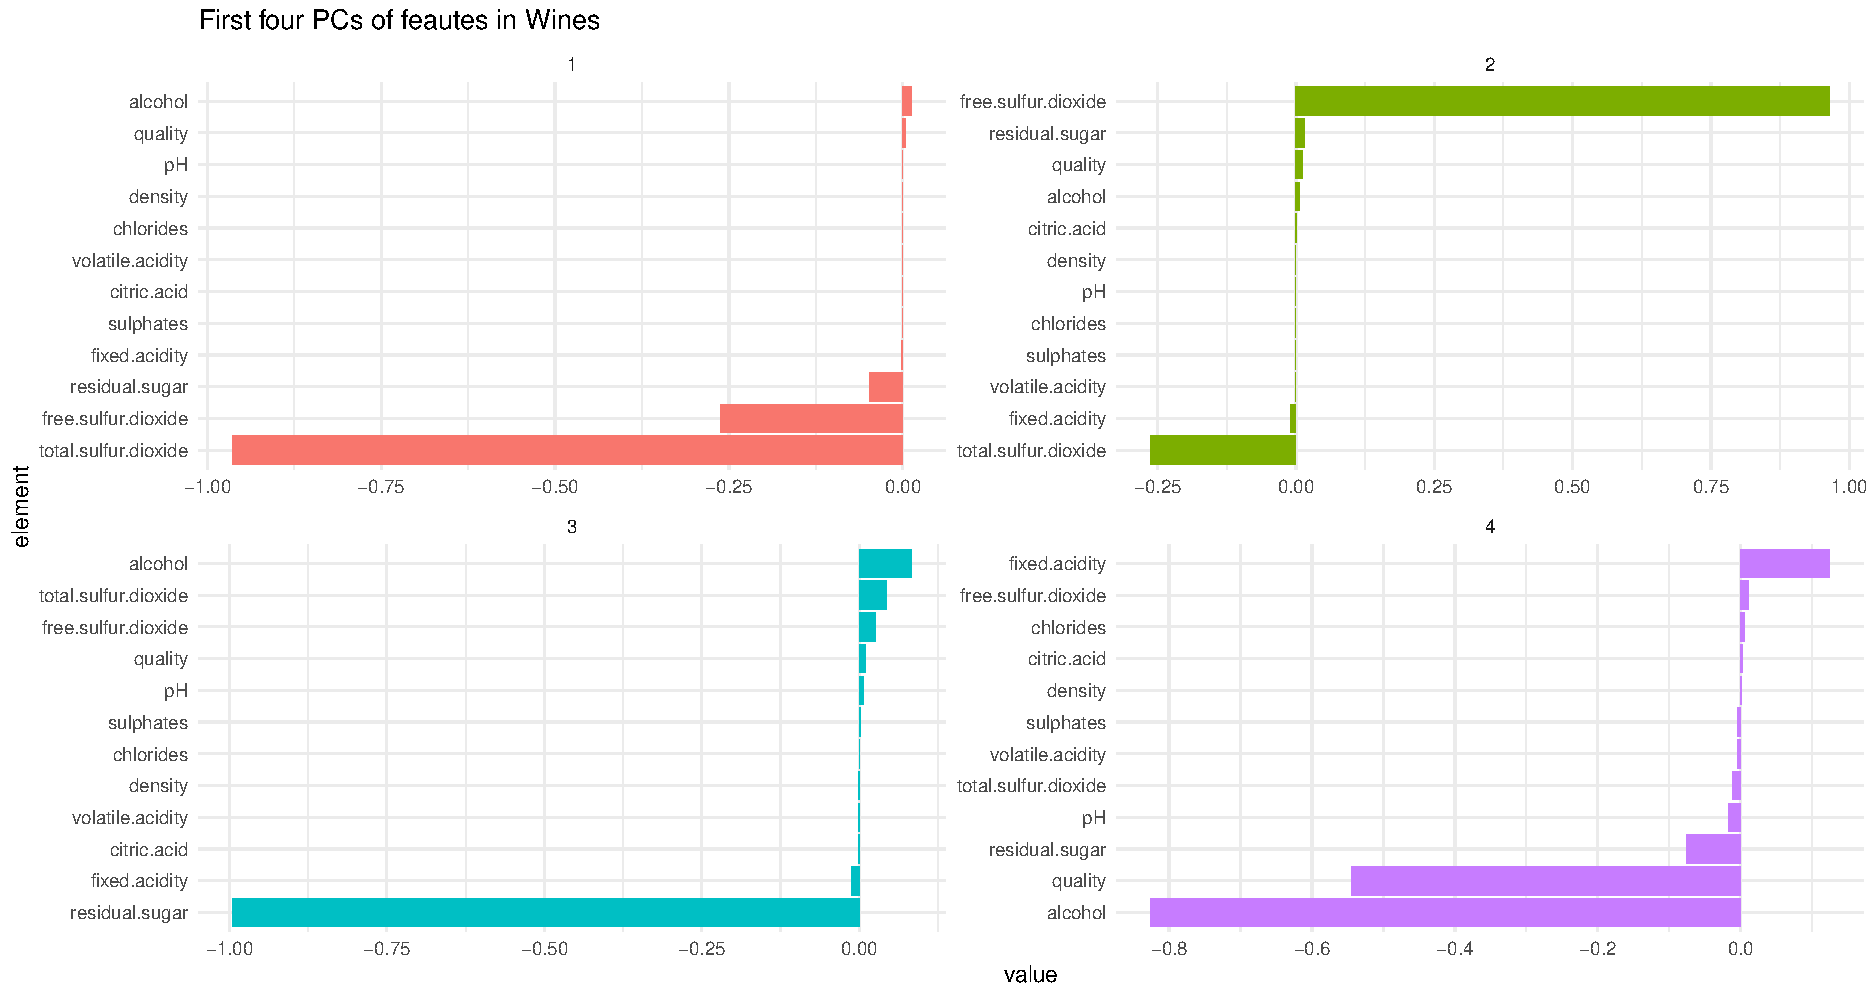
\includegraphics[width=.8\textwidth]{./output/1.b.pca-features.pdf}
\caption{First four principal component loading scores per feature}
\label{fig:uni}
\end{center}
};

\node (n1c) [text width=0.48\textwidth, align = justify, anchor = north west, inner sep = 0] at ($ (n1b.south west) + (0, 0) $)
{
\mysection{Model}
%-------------------

\begin{tikzpicture}[x=2pt,y=2.3pt,yscale=-1,xscale=1]
%\begin{tikzpicture}[scale=\tikzscale]
%uncomment if require: \path (0,329); %set diagram left start at 0, and has height of 329
%Shape: Rectangle [id:dp6981379495439248]
\draw (11,142.63) -- (50.93,142.63) -- (50.93,260.63) -- (11,260.63) -- cycle ;
%Straight Lines [id:da21346322770194326]
\draw (50.93,201.63) -- (106.93,201.63) ;
\draw [shift={(108.93,201.63)}, rotate = 180] [color={rgb, 255:red, 0; green, 0; blue, 0 } 
][line width=0.75] (10.93,-3.29) .. controls (6.95,-1.4) and (3.31,-0.3) .. (0,0) .. controls (3.31,0.3) and (6.95,1.4) .. (10.93,3.29) ;
%Shape: Rectangle [id:dp29000115422593087]
\draw (108,125.63) -- (147.93,125.63) -- (147.93,276.63) -- (108,276.63) -- cycle ;
%Shape: Rectangle [id:dp3116438864292579]
\draw (209,128.63) -- (248.93,128.63) -- (248.93,276.63) -- (209,276.63) -- cycle ;
%Shape: Rectangle [id:dp5504046010346768]
\draw (308,92.63) -- (347.93,92.63) -- (347.93,309.63) -- (308,309.63) -- cycle ;
%Shape: Rectangle [id:dp2926920978374945]
\draw (412,95.63) -- (451.93,95.63) -- (451.93,309.63) -- (412,309.63) -- cycle ;
%Shape: Rectangle [id:dp43902801324987895]
\draw (512,156.63) -- (551.93,156.63) -- (551.93,248.63) -- (512,248.63) -- cycle ;
%Straight Lines [id:da19613399481990768]
\draw (149.93,202.63) -- (205.93,202.63) ;
\draw [shift={(207.93,202.63)}, rotate = 180] [color={rgb, 255:red, 0; green, 0; blue, 0 } 
][line width=0.75] (10.93,-3.29) .. controls (6.95,-1.4) and (3.31,-0.3) .. (0,0) .. controls (3.31,0.3) and (6.95,1.4) .. (10.93,3.29) ;
%Straight Lines [id:da7665092917579182]
\draw (248.93,202.63) -- (304.93,202.63) ;
\draw [shift={(306.93,202.63)}, rotate = 180] [color={rgb, 255:red, 0; green, 0; blue, 0 } 
][line width=0.75] (10.93,-3.29) .. controls (6.95,-1.4) and (3.31,-0.3) .. (0,0) .. controls (3.31,0.3) and (6.95,1.4) .. (10.93,3.29) ;
%Straight Lines [id:da00009484808513526843]
\draw (350.93,203.63) -- (406.93,203.63) ;
\draw [shift={(408.93,203.63)}, rotate = 180] [color={rgb, 255:red, 0; green, 0; blue, 0 } 
][line width=0.75] (10.93,-3.29) .. controls (6.95,-1.4) and (3.31,-0.3) .. (0,0) .. controls (3.31,0.3) and (6.95,1.4) .. (10.93,3.29) ;
%Straight Lines [id:da5648066531472558]
\draw (450.93,202.63) -- (506.93,202.63) ;
\draw [shift={(508.93,202.63)}, rotate = 180] [color={rgb, 255:red, 0; green, 0; blue, 0 } ][line width=0.75] (10.93,-3.29) .. controls (6.95,-1.4) and (3.31,-0.3) .. (0,0) .. controls (3.31,0.3) and (6.95,1.4) .. (10.93,3.29) ;
% Text Node
\draw (7,104) node [anchor=north west][inner sep=0.75pt] [align=left] {Dense};
% Text Node
\draw (104,91) node [anchor=north west][inner sep=0.75pt] [align=left] {Dense};
% Text Node
\draw (211,84) node [anchor=north west][inner sep=0.75pt] [align=left] {\begin{minipage}[lt]{24.81pt}\setlength\topsep{0pt}
\begin{center}
MC\\Drop
\end{center}
\end{minipage}};
% Text Node
\draw (414,49) node [anchor=north west][inner sep=0.75pt] [align=left] {\begin{minipage}[lt]{24.81pt}\setlength\topsep{0pt}
\begin{center}
MC\\Drop
\end{center}
\end{minipage}};
% Text Node
\draw (304,65) node [anchor=north west][inner sep=0.75pt] [align=left] {Dense};
% Text Node
\draw (510,134) node [anchor=north west][inner sep=0.75pt] [align=left] {Dense};
% Text Node
\draw (21,237.4) node [anchor=north west][inner sep=0.75pt] {$12$};
% Text Node
\draw (118,253.4) node [anchor=north west][inner sep=0.75pt] {$32$};
% Text Node
\draw (219,254.4) node [anchor=north west][inner sep=0.75pt] {$32$};
% Text Node
\draw (313,288.4) node [anchor=north west][inner sep=0.75pt] {$160$};
% Text Node
\draw (417,289.4) node [anchor=north west][inner sep=0.75pt] {$160$};
% Text Node
\draw (526,226.4) node [anchor=north west][inner sep=0.75pt] {$3$};
% Text Node
\draw (161,10) node [anchor=north west][inner sep=0.75pt] [font=\large] [align=left] {\textbf{Monte Carlo Dropout BNN}};
\end{tikzpicture}

\textbf{Dropout layer}
\begin{itemize}
\item Dropout layers work only during training.
\item They randomly ignore a percentage of neurons and their connections.
\item Randomly means, by random draws of a Bernoulli distribution.
\item This process generates a \textbf{deterministic} prediction.
\end{itemize}

\textbf{Monte Carlo Dropout layer}
\begin{itemize}
\item MC dropout is a wrapper of the simple dropout function.
\item It preserves the random dropout of neurons at testing time.
\item This process generates a \textbf{stochastic} prediction.
\end{itemize}

%-------------------
};

\node (n20) [text width=0.48\textwidth
, align = justify, anchor = north west, inner sep = 0] at ($ (n1.north east) + (2em, 0) $)
{
	\mysection{Validation}

\textbf{Explanation of model fitting}
\begin{itemize}
\item There exist a lot of variance in the prediction due to randomness.
\item The validation and the training accuracy are at the same level.
\end{itemize}

\begin{center}
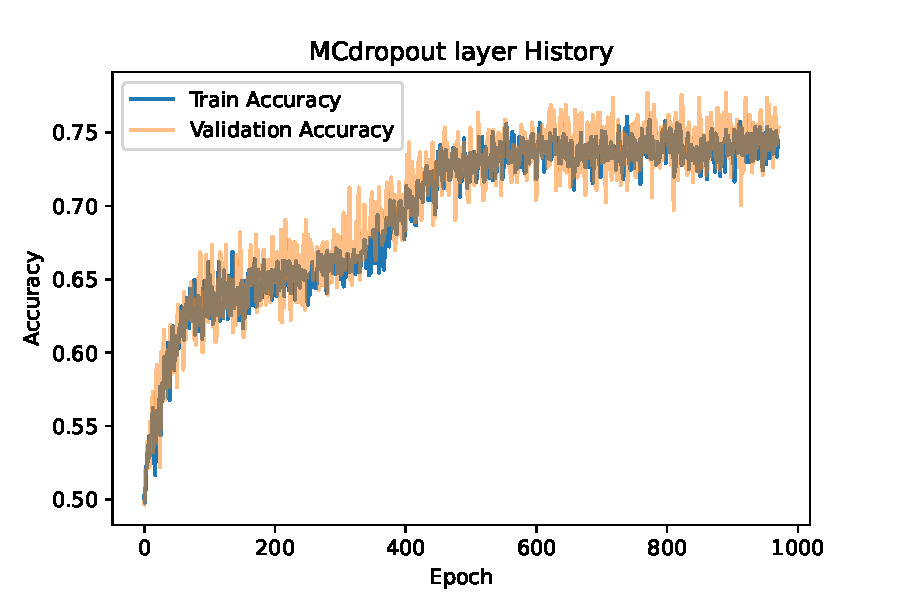
\includegraphics[width=.7\textwidth]{./output/2.d.history-mcdrop.pdf}
\caption{Epochs training}
\label{fig:uni}
\end{center}
\vspace{2em}
};

\node (n21) [text width=0.48\textwidth, align = justify, anchor = north west, inner sep = 0] at ($(n20.south west) + (0, 0) $)
{
\mysection{Explanation}

\textbf{Shap Values}
\begin{itemize}
\item The most influential features in descending order.
\item Further granularity, fixed acidity low, then low impact on prediction class 1.
\item Prior knowledge gained in EDA is confirmed in model explanation by SHAP.
\end{itemize}

\vspace*{1em}
\centering
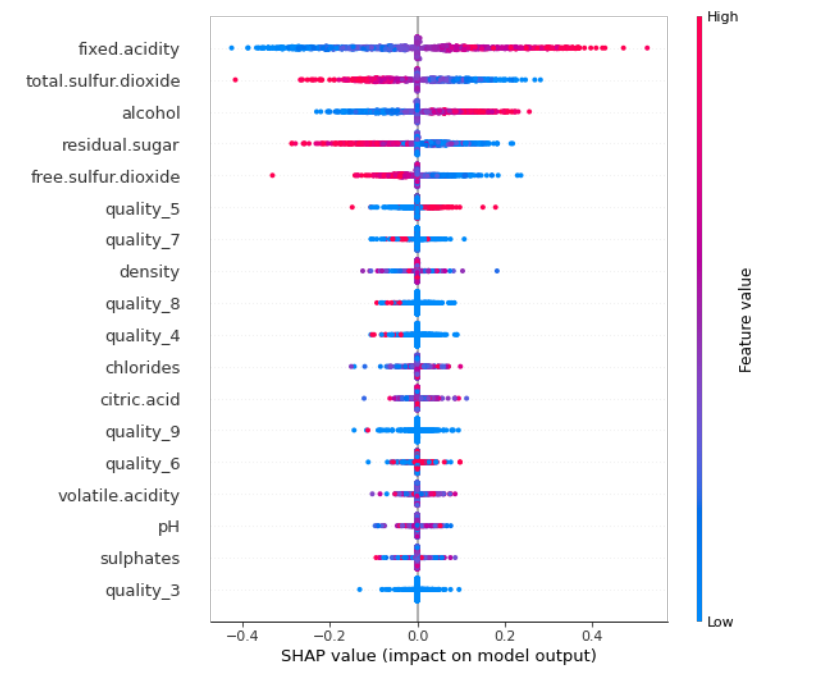
\includegraphics[width=.7\textwidth]{./output/shap.png}
\caption{Shapley values per feature value for wine type $2$}
\label{fig:uni}
\vspace{2em}

};


\node (n22) [text width=0.48\textwidth, align = justify, anchor = north west, inner sep = 0] at ($ (n21.south west)$)
{
\mysection{Entropy}

{

\textbf{Defintion}\\
Informational entropy or Shannon entropy:

\begin{equation}
H(x) = - \sum_{(k=1)}^K p(X=k)log_2(X=k)
\end{equation}

\begin{itemize}
\item We have $K=3$ classes in this exercise.
\item When the algorithm predicts $\frac{1}{3}$ for all three classes, then the entropy is maximized.
\item This is because the uniform distribution is the most uncertain. 
\item A distribution where all the mass is in exatly one outcome, has minimum entropy.
\end{itemize}

\textsf{Entropy Example}
\centering
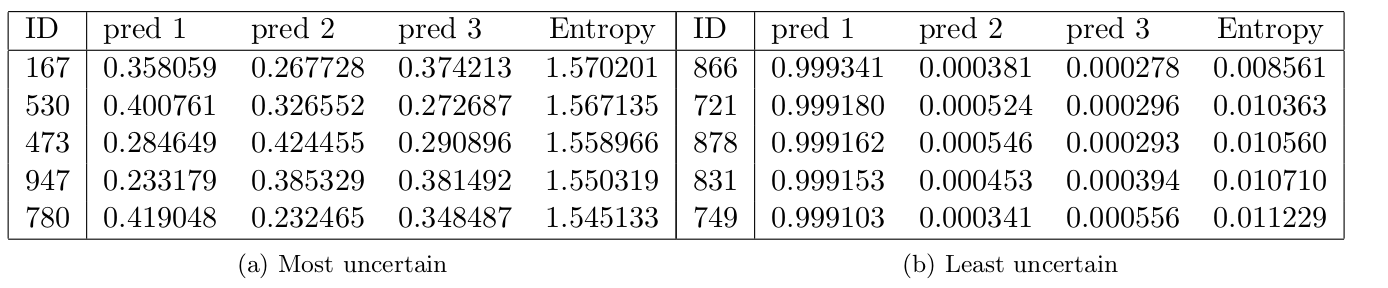
\includegraphics[width=\textwidth]{./output/table.png}
\caption{Sample outcome of Anomalies}
\label{fig:uni}
\vspace{.5em}
By setting a threshold $t$ we can create a \textbf{binary measure of uncertainty}.
\[ 
f(\text{entropy})= \left\{
\begin{array}{ll}
      1, & \text{entropy} \geq t \\
      0, & \text{entropy} < t\\
\end{array} 
\right. 
\]

}

};

%%%%%%%%%%%%%%%%%%%%%%%%%%%%%%%%%%%%%%%%%%%
%
% Decorative lines.
%
%%%%%%%%%%%%%%%%%%%%%%%%%%%%%%%%%%%%%%%%%%%



% this is a separating line between  the two text columns
\node (l1) at ($ (n1.north east) + (1em, 0) $) {};
\node (l2) at ($ (n1c.south east) + (1em, 0) $) {};
\draw[black] (l1) -- (l2);


%\node (l3) at ($ (n7.north east) + (0.025\linewidth, 0) $) {};
%\node (l4) at ($ (l2) + (0.35\linewidth, 0) $) {};
%\draw[black] (l3) -- (l4);


\end{scope}
\end{tikzpicture}

\end{poster}

\end{document}
